

\chapter{Aerial Mapping and Photogrametry} \label{chap:AerialMapping}



\section{The need for mapping the land}
The first known map (actually a painting of a city) dates up to the 7th millenium BCE,\cite{map1}, while the oldest surviving world maps are from 9th centursy BCE Babylonia\cite{map2}.

In the past, maps were used mostly for localization and navigation %$^{\text{[citation needed]}}$ \todo{citation needed}
, and were made without special tools, mainly by sight. During the Age of Exploration, new tools such as the sextant and magnetic compass helped improve accuracy, while remaining as a navigational tool.

On the last centuries, maps began being used to precisely map properties, natural landscapes, and cities, and used as a tool of government\cite{mapgovernment}. Mapping properties, for example, requires high dimensional accuracy, hard to get with regular tools. This is usually the job of land surveyors, professionals who use a multitude of tools, such as total stations, robotic total stations, GPS receivers, retro reflectors, 3D scanners, radios, handheld tablets, digital levels, subsurface locators, drones, GIS, and surveying software.


\section{Aerial Mapping}
Aerial mapping consists of using photographs taken from the air, usually with the camera facing straight downwards, correcting the perspective transformation, and assembling them into an orthomosaic, as seen on Figure \ref{fig:orthomosaic}.

\begin{figure}
\centering
  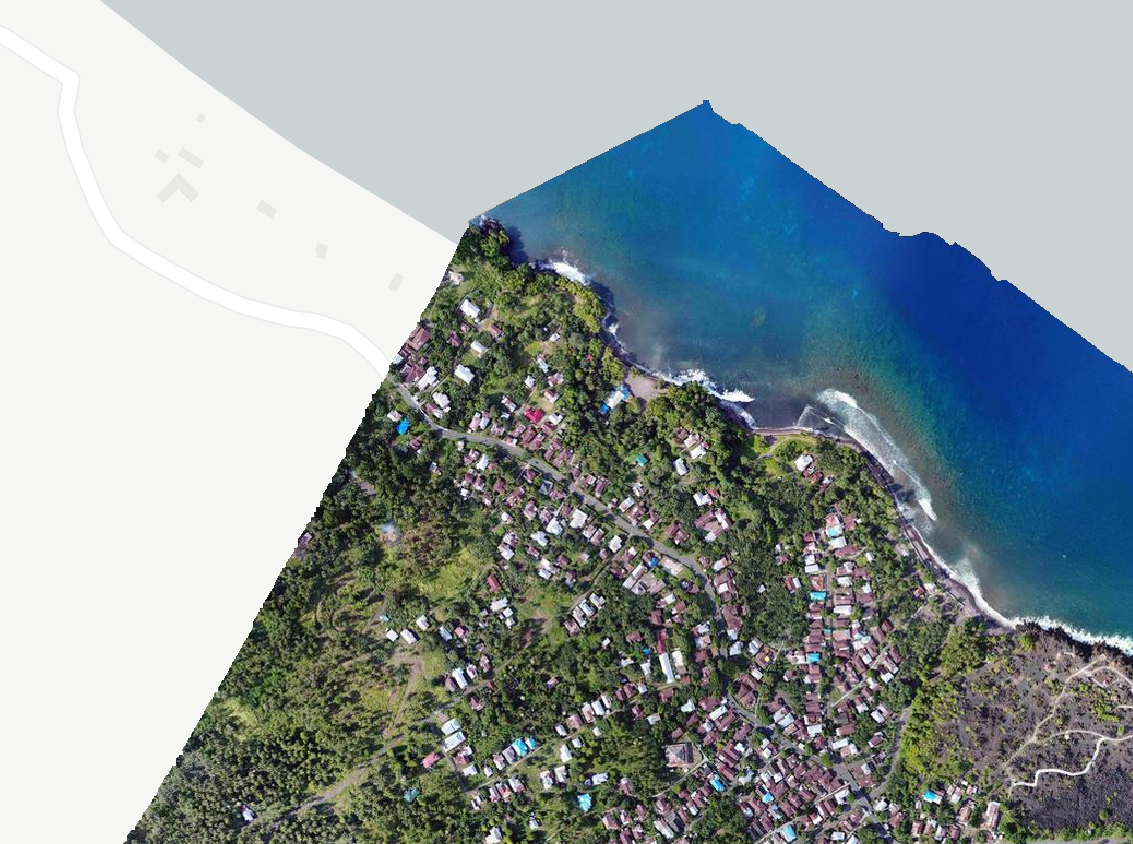
\includegraphics[width=\linewidth]{figs/orthomosaic.png}
  \caption{Orthomosaic. source: Indonesian Redcross/OpenAerialMap}
  \label{fig:orthomosaic}
\end{figure}


\section{Aerophotogrammetry}

Aerophotogrammetry takes the job on step further. 
%
By knowing the camera's intrinsic parameters, software are capable of matching a number of pictures, detecting features on the environment, and locating the point used to take each of the pictures, this process is called multi-view stereo. 
%
With this information, it's possible to rebuild in 3D most of the environments, enabling the operator to interact with the area as a 3D mesh.
%
By using precise GPS information(such as RTK/PPK data, or total stations) or known landmarks, it's possible to accurately measure distances, areas, volumes, angles and elevations, simplifying the surveyors' job.
%
Aerophotogrametry can also be used to rebuild in 3D buildings and other structures, enabling precise calculations of volume and distances, allowing the use of 3D models on CAD software for faster and easier construction and planning.
%
It allows, for example, the calculation of displaced volume on a quarry, or how much landfill is required to level some terrain.
%

The results of an open-source multi-view stereo pipeline implementation usint openMVS\cite{openmvs} and openMVG\cite{openmvg} can be seen on figures \ref{fig:cameras} and \ref{fig:church}. 
%
On figure \ref{fig:cameras} the software shows the cameras found, and their relative positions on the map. 
%
The orange areas are locations not covered by the cameras. 
%
It is important to notice that, as the coverage is does not catch every angle of the structures, some deformations are expected, especially on hidden areas. 
%
Figure \ref{fig:church} shows the rebuilt and textured 3D model.
 
 \begin{figure}
\centering
  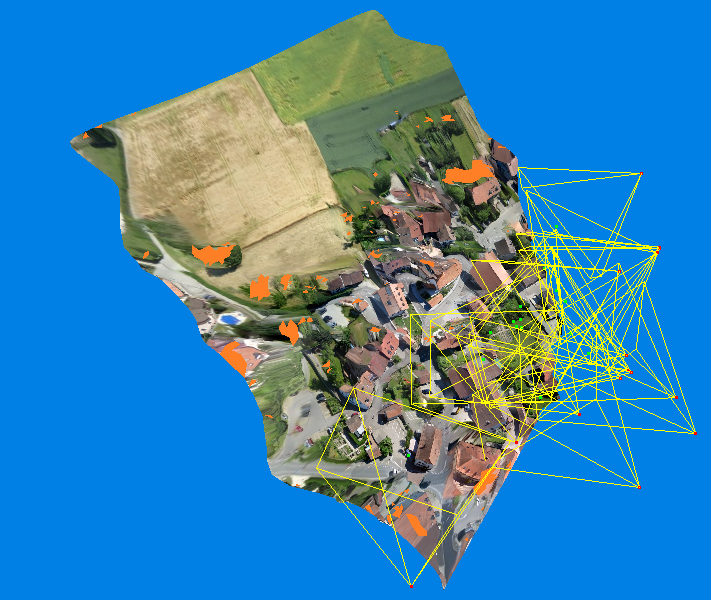
\includegraphics[width=\linewidth]{figs/cameras.png}
  \caption{Identified camera positions on "Oblique mapping of a village" dataset }
  \label{fig:cameras}
\end{figure}


 \begin{figure}
\centering
\begin{subfigure}{.5\textwidth}
  \centering
  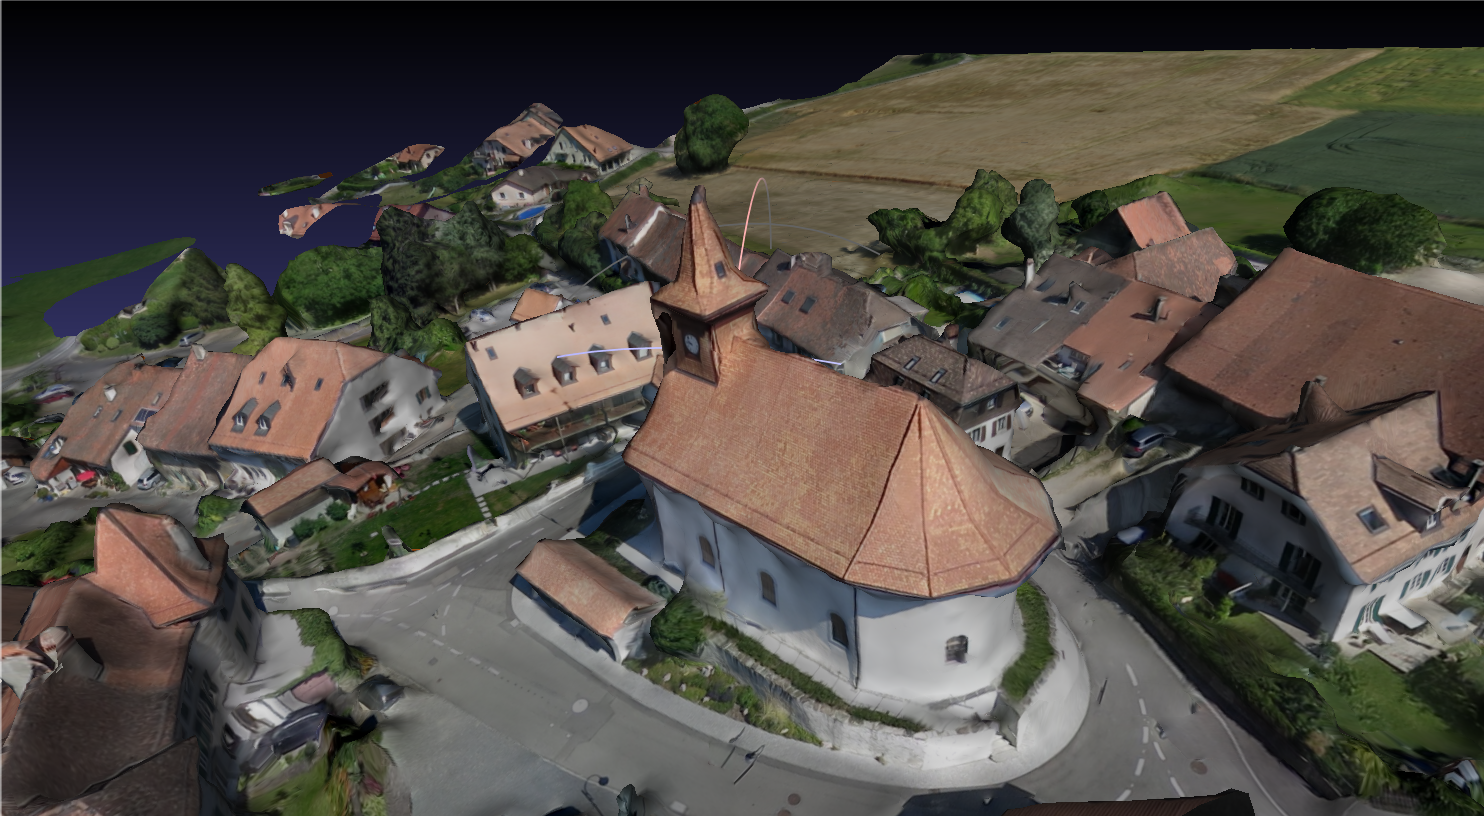
\includegraphics[width=\linewidth]{figs/church1.png}
  %\caption{Todos os passos do Nelder-Mead}
  
\end{subfigure}%
\begin{subfigure}{.5\textwidth}
  \centering
  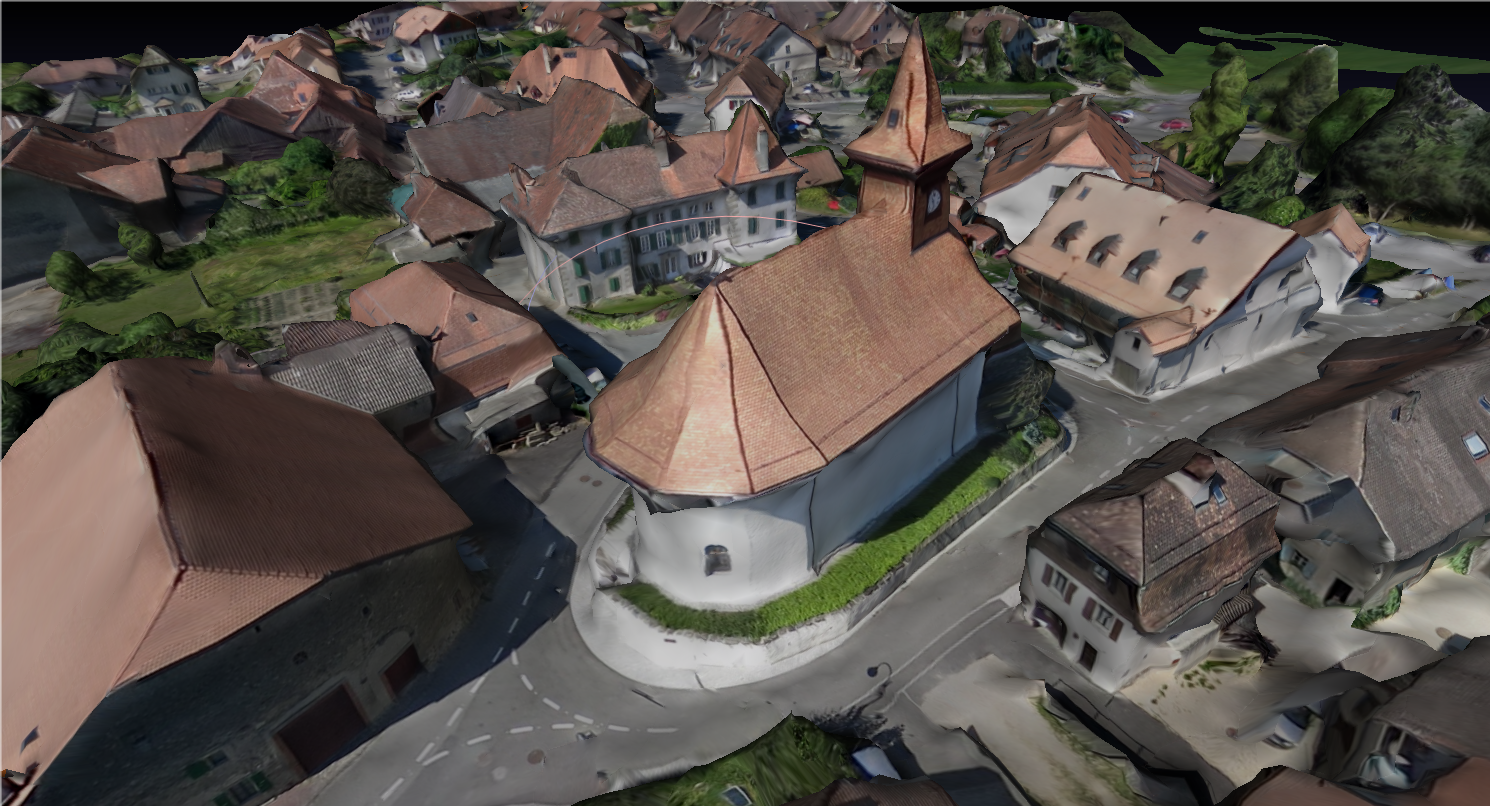
\includegraphics[width=\linewidth]{figs/church2.png}
  %\caption{Pontos avaliados pelo Nelder-Mead aplicado em um parabolóide.}

\end{subfigure}
\caption{3D reconstruction visualization of the "Oblique mapping of a village" dataset.}
\label{fig:church}
\end{figure}

